
%\addcontentsline{toc}{chapter}{Anhang}
\cftaddtitleline{toc}{chapter}{Anhang}{}
\pagenumbering{Roman}
\appendix


\chapter{Ausschreibung Bachelorarbeit}
\label{Ausschreibung} 

\begin{figure}[h]
    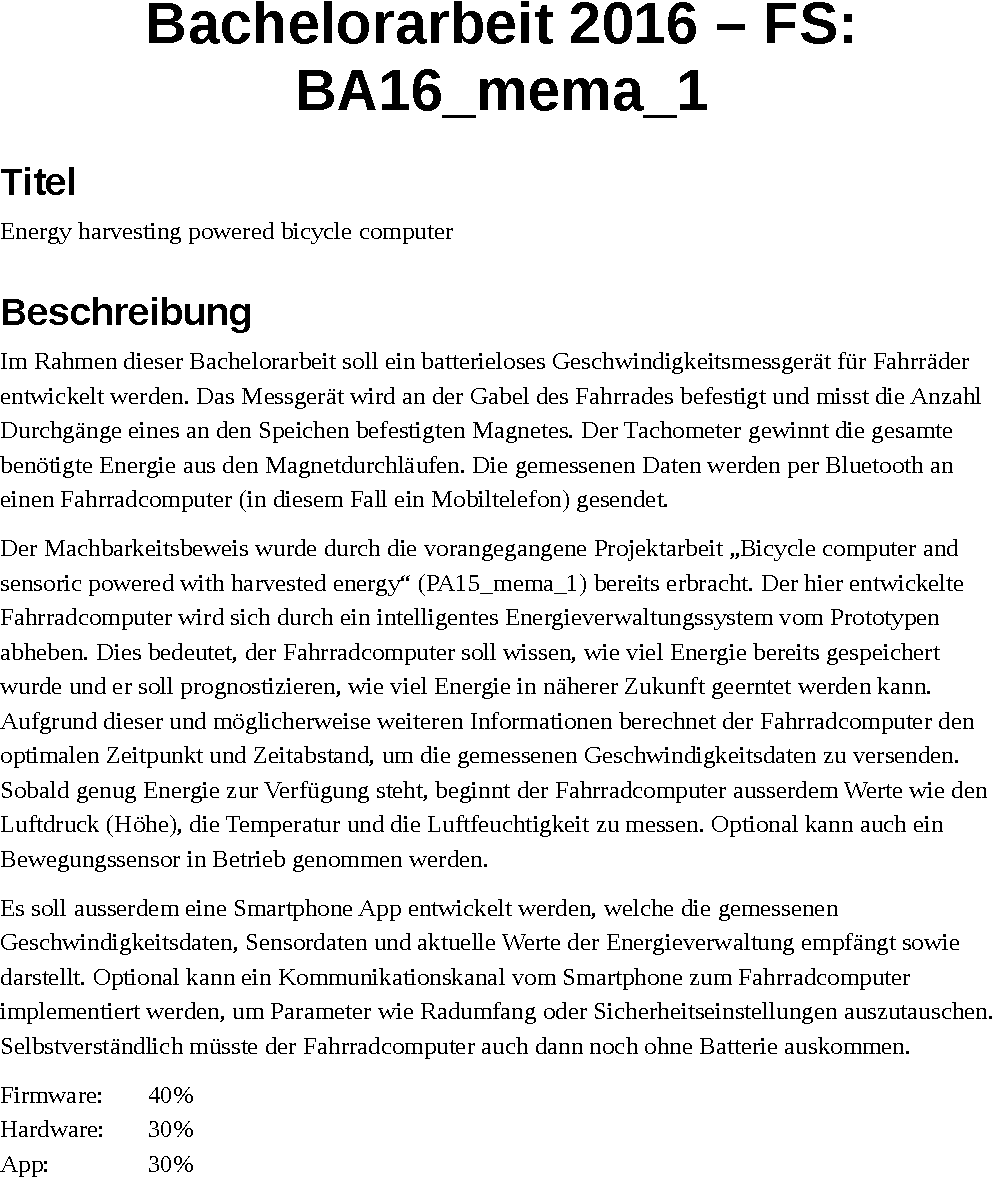
\includegraphics [width=0.8\textwidth] {7Anhang/docs/Ausschreibung-cropped.pdf} 
     \caption{Offizielle Ausschreibung der Arbeit}
\end{figure}



\chapter{Blockdiagramm EM8500}
\label{anhang_em8500} 

\begin{figure}[h]
    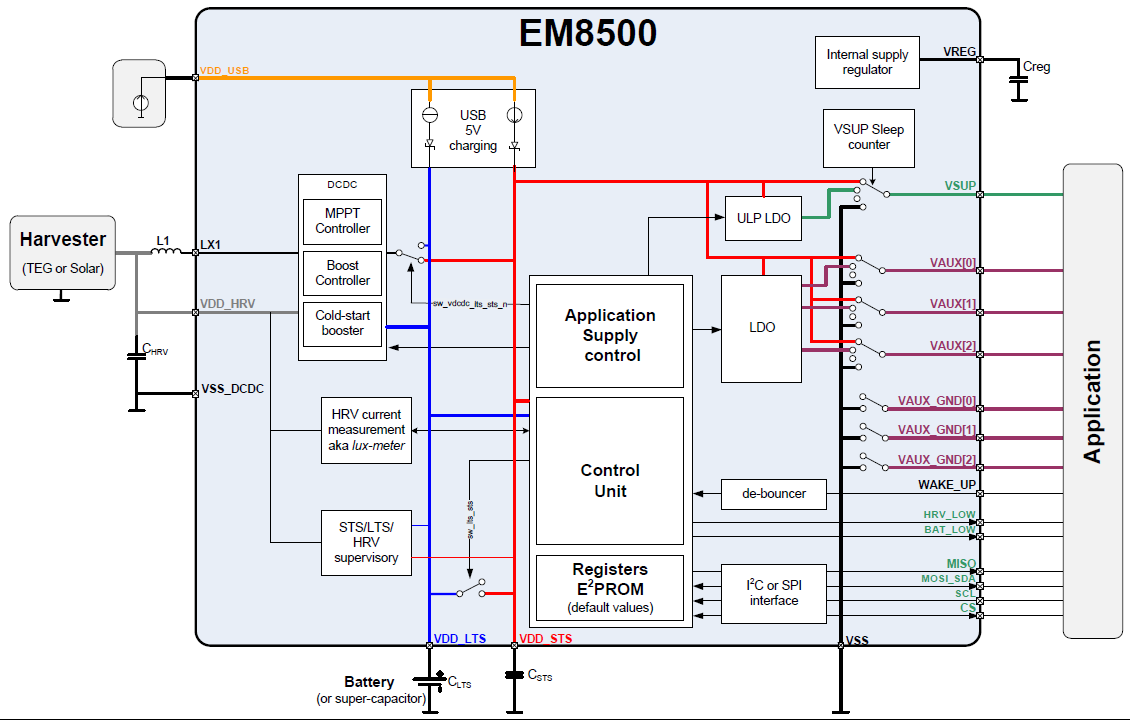
\includegraphics [width=1\textwidth]{7Anhang/imag/blockdiagrammEm8500.png} 
     \caption{Blockschema Sensortag}
\end{figure}



\chapter{Funktionsblöcke des TI-SensorTags}
\label{anhang_sensortag} 

\begin{figure}[h]
    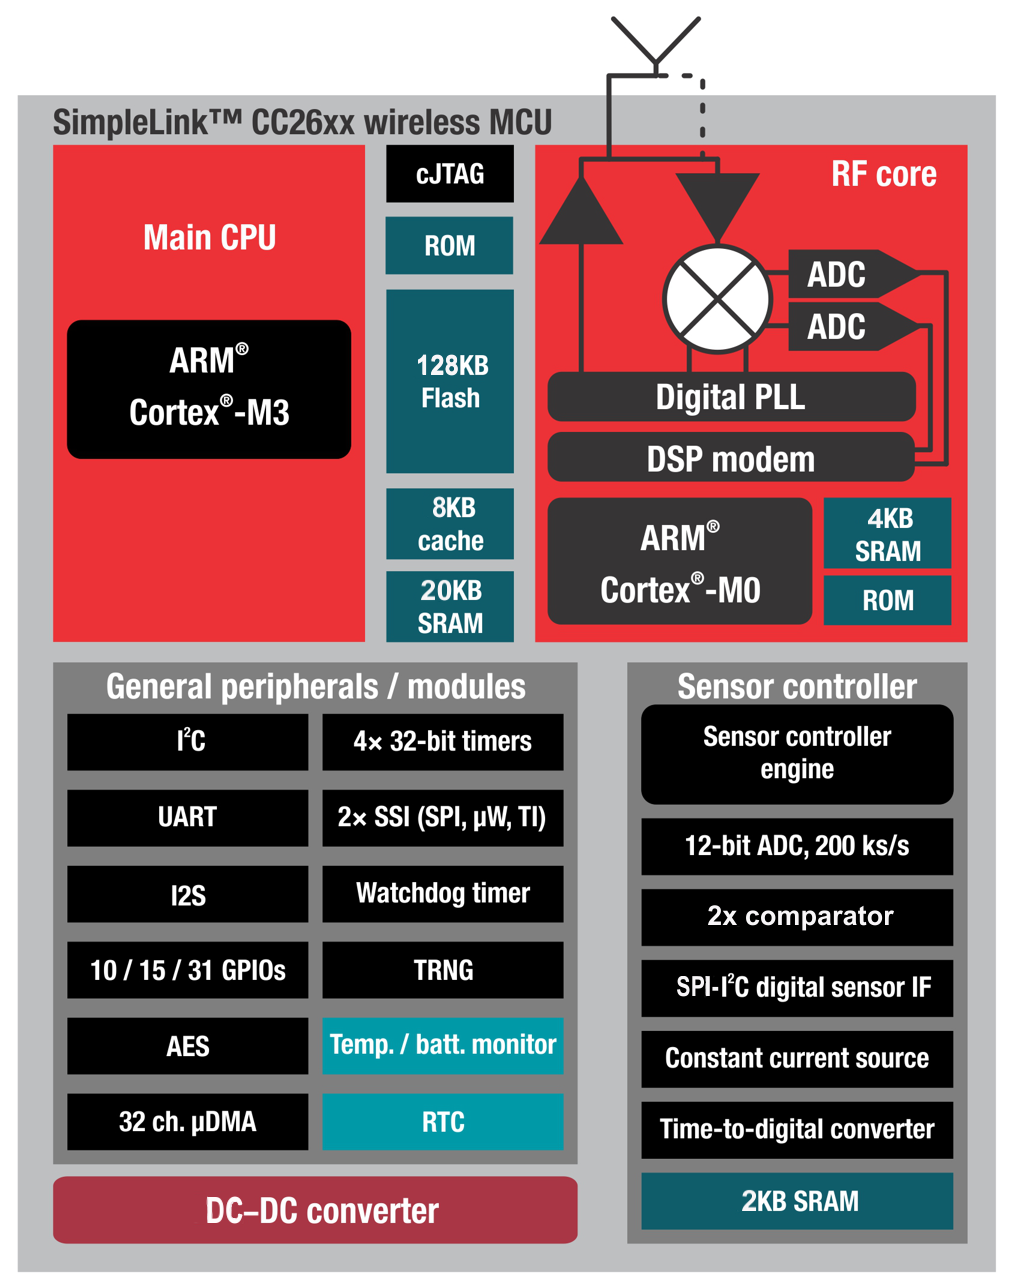
\includegraphics [width=0.7\textwidth]{7Anhang/imag/CC26xx_Block_Diagram.png} 
     \caption{Blockschema TI-SensorTag aus \cite{Sensortag_Datasheet}, S.\,3}
\end{figure}


%\chapter{Supply System beim TI-SensorTag}
%\label{anhang_sensortag_supply} 
%
%\begin{figure}[h]
%    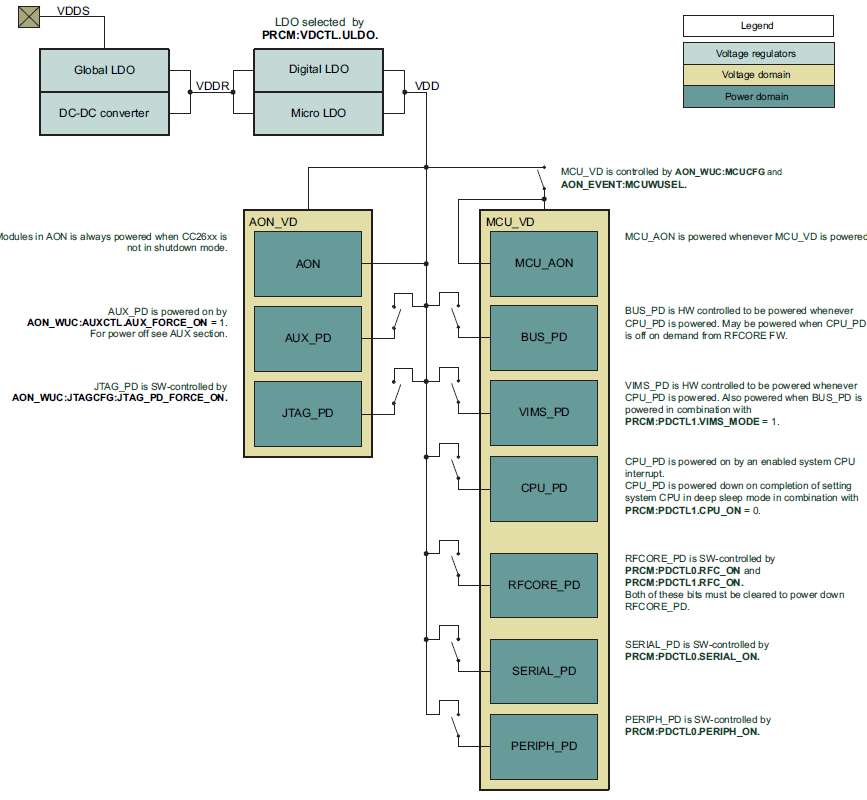
\includegraphics [width=0.7\textwidth]{7Anhang/imag/powerdomain_1.png} 
%    \caption{Abbildung aus \cite{Sensortag_Manual}, S.\,416}
%    \label{a_supply}
%\end{figure}


\chapter{Digital Power Partitioning beim TI-SensorTag}
\label{anhang_sensortag_PowerDomain} 

\begin{figure}[h]
    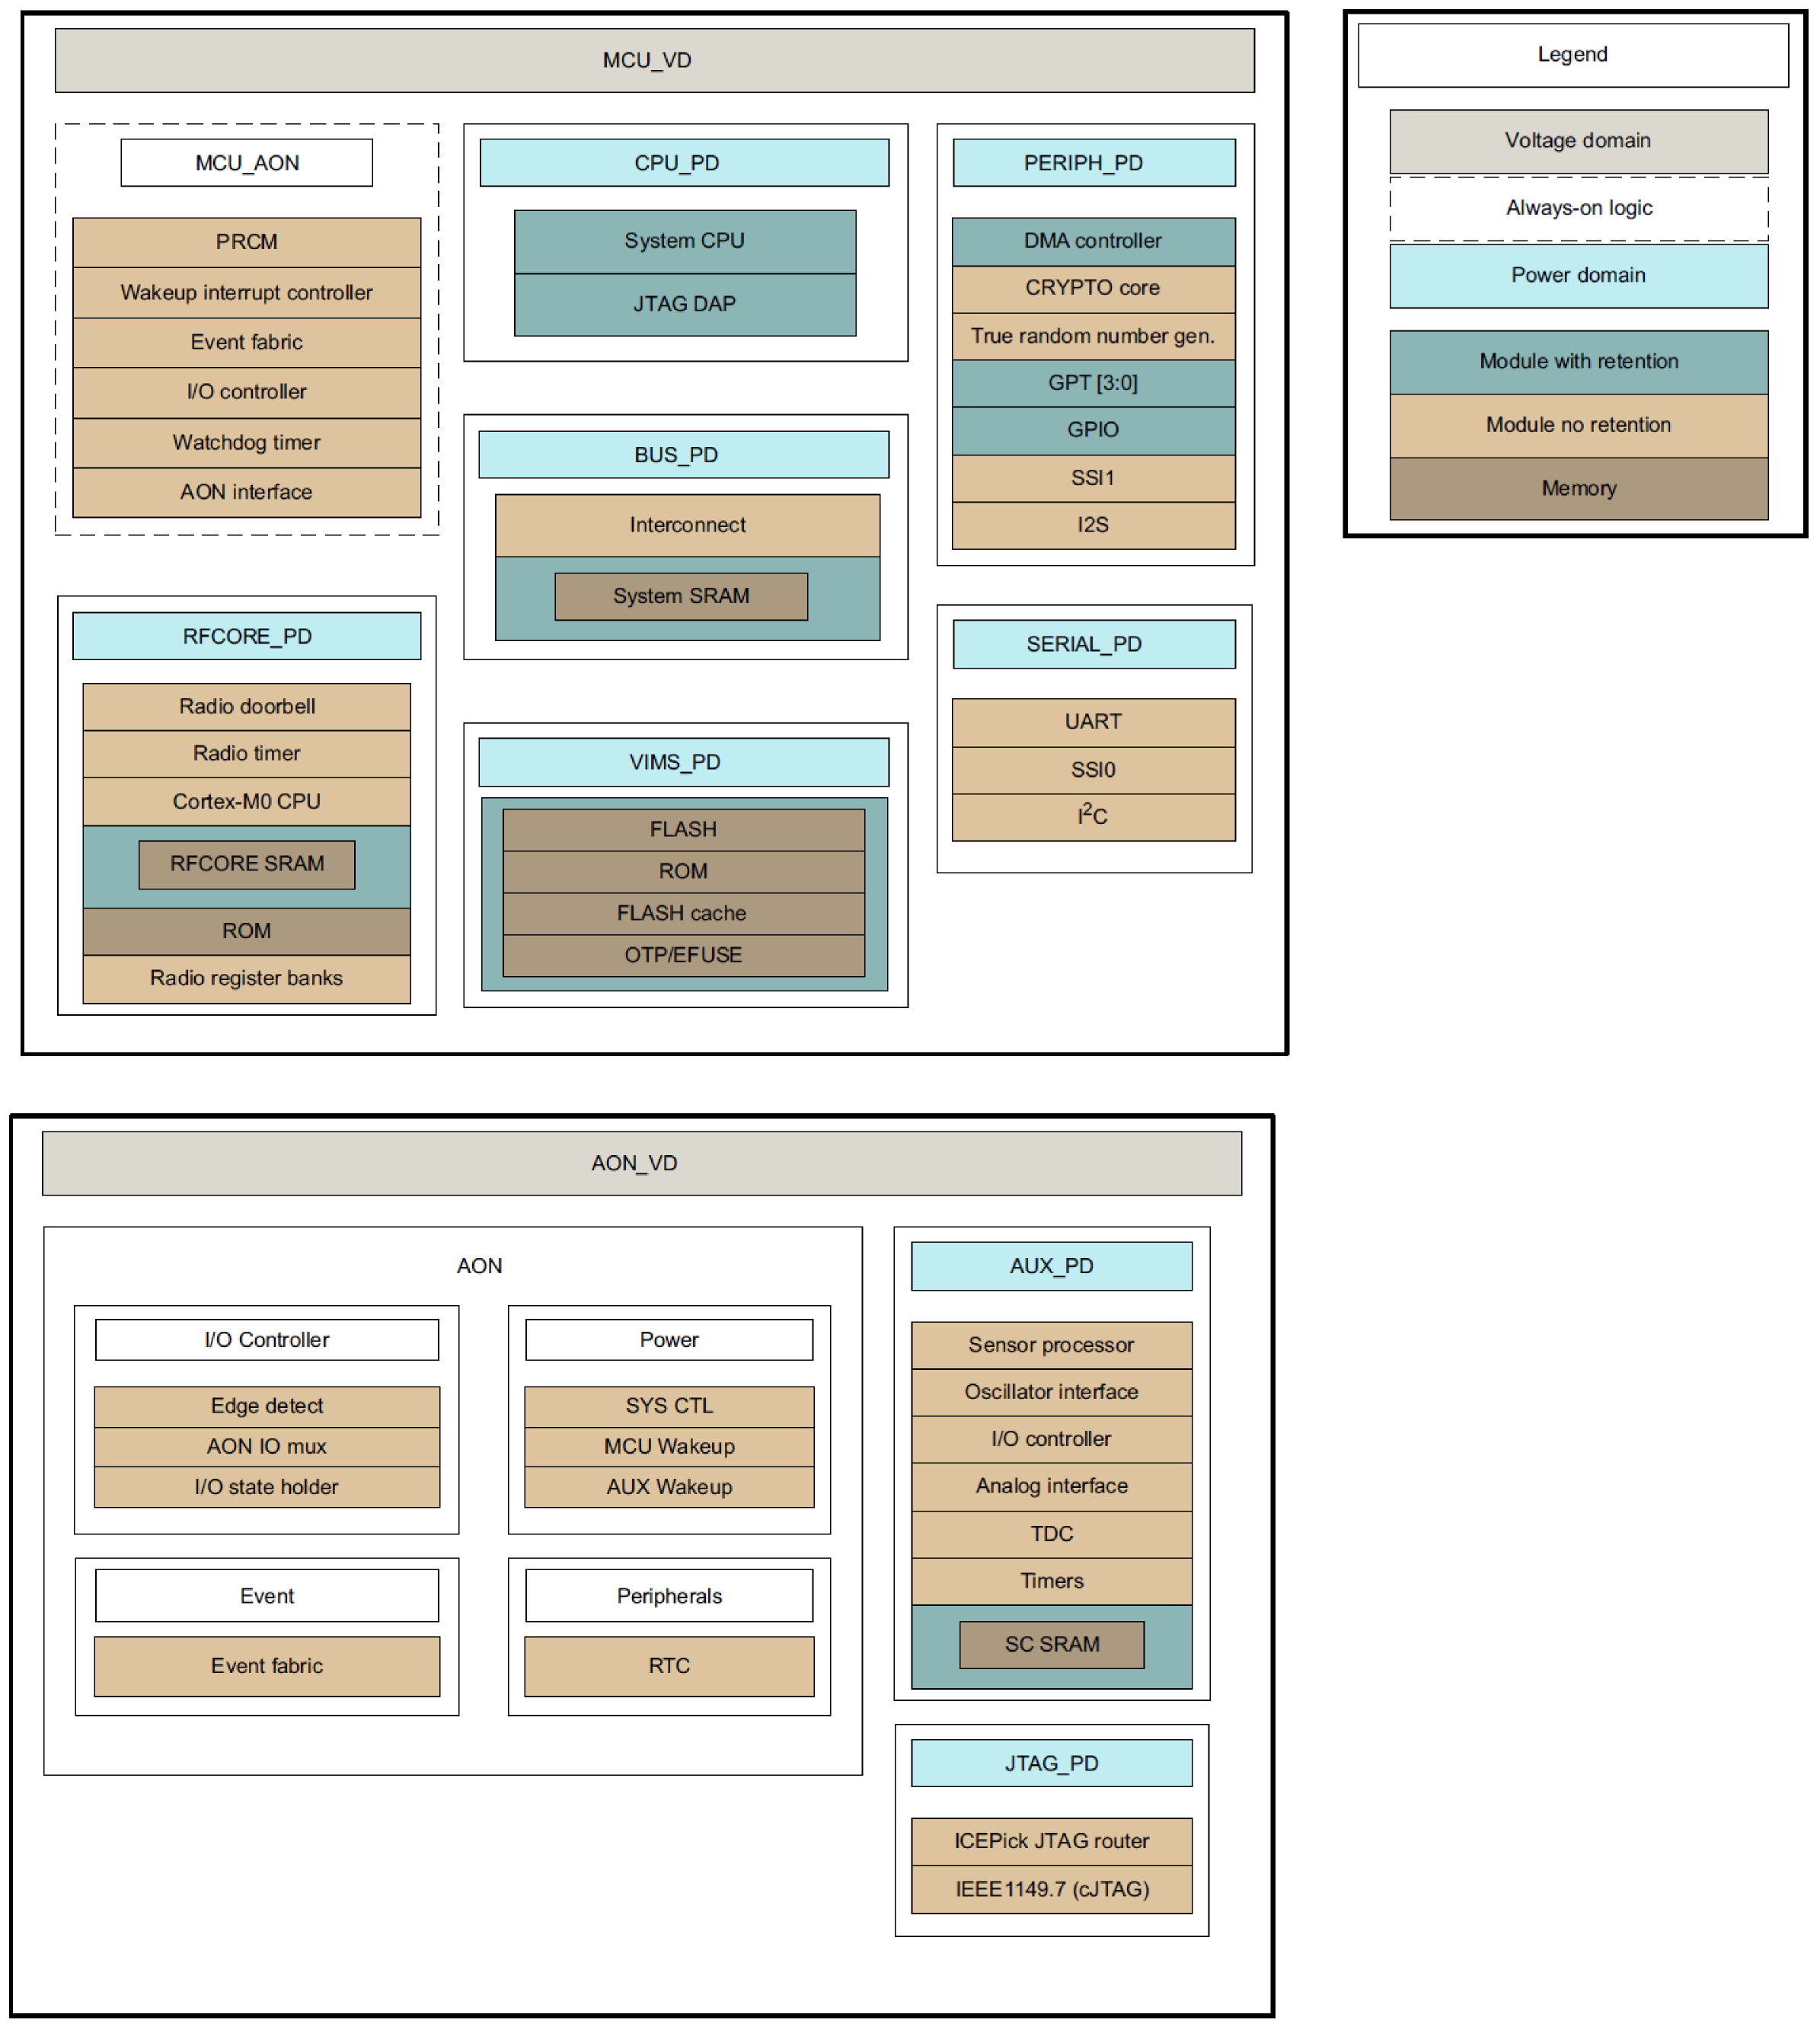
\includegraphics [width=0.8\textwidth]{7Anhang/imag/powerDomain_2.png} 
     \caption{Abbildung aus \cite{Sensortag_Manual}, S.\,418}
     \label{a_powerdomain}
\end{figure}

\chapter{Messaufbau}
\label{messaufbau}
Problematisch war, dass die Messresultate mit dem Fahrrad nicht reproduzierbar waren, daher wurde eine Radimitation erarbeitet. Herr Erich Ruff hat einen Aubau entwickelt, welcher über einen Elektromotor angetrieben wurde, damit konnte die Geschwindigkeit relativ konstant gehalten werden. Die Toleranz der Geschwindigkeit lag bei +/- 1 km/h, was eine grosse Verbesserung gegenüber der bisherigen Vorgehensweise war. Die Radimitation bestand aus nur einer Speiche, welche nur eine einfache Alustange war. An dieser Alustange waren mehrere Löcher zur Befestigung des Topfmagneten vorhanden.

\begin{figure}[ht]
    \includegraphics [width=1\textwidth]{7Anhang/imag/Messaufbau}
	\caption{Messaufbau während der Inbetriebnahme des Prototypen}
	\label{messaufbau_anhang}
\end{figure}

Der Radimitation ist ein Tachometer angehängt, der die aktuelle Geschwindigkeit anzeigt. Der Tachometer ist vom Hersteller Sigma Sport, die genaue Bezeichnung Lautet Sigma Sport Baseline 500. Dieser Tachometer wurde im Jahr 1999 hergestellt, funktioniert jedoch nach wie vor einwandfrei. Im Verlauf der Entwicklung wurde entschieden, dass zwei Magnete im Abstand von 180 Grad angebracht werden. Diese Entscheidung wurde getroffen, um die Energiegewinnung zu maximieren, es wurde jedoch ebenfalls entschieden, dass nicht mehr als zwei Magnete montiert werden sollen. Das Erscheinungsbild des Fahrrads würde damit sehr beeinträchtigt und die Bremswirkung würde mit vielen Magneten sicherlich zum Tragen kommen.

Alle Messungen werden mit einem Radumfang von 2.04 m ausgeführt, der Magnet befand sich 25 cm vom Zentrum der Radsimulation entfernt. Den Einfluss des Abstands kann aus dem Messprotokoll vom 06. Mai 2016 entnommen werden.

\chapter{Messprotokolle per Datum und Messobjekt}
\label{uebersicht_messprotokolle}

\label{tabelle_uebersicht_messprotokolle}
\begin{itemize}
\item 26. Februar 2016, \emph{Harvesterausgang Elko}\\
Messprotokoll\_Kondensator\_Ausgang\_Harvesterschaltung.pdf
\item 14. März 2016, \emph{Gleichrichter}\\
Messprotokoll\_Optimierung\_Gleichrichter\_1.pdf
\item 26. Februar 2016, \emph{Harvesterausgang Elko}\\
Messprotokoll\_Kondensator\_Ausgang\_Harvesterschaltung.pdf
\item 14. März 2016, \emph{Spule}\\
Messprotokoll\_Optimierung\_Spule.pdf
\item 14. März 2016, \emph{Gleichrichter}\\
Messprotokoll\_Optimierung\_Gleichrichter\_1.pdf
\item 14. März 2016, \emph{Gleichrichter}\\
Messprotokoll\_Optimierung\_Gleichrichter\_2.pdf
\item 14. März 2016, \emph{Spannungsbegrenzung}\\
Messprotokoll\_Optimierung\_Limiter.pdf
\item 19. März 2016, \emph{Harvesterausgang}\\
Messprotokoll\_Leistungskennlinie\_Harvester\_versch\_Harvester.pdf
\item 30. März 2016, \emph{EM8500-Chip-Ausgang}\\
Messprotokoll\_Leistungskennlinie\_Harvester\_fliegender\_Aufbau.pdf
\item 14. April 2016, \emph{Spule und Magnete}\\
Messprotokoll\_Optimierung\_Spule\_versch\_Spulen\_und\_Magnete.pdf
\item 14. April 2016, \emph{Harvesterausgang}\\
Messprotokoll\_Leistungskennlinie\_Harvester\_Prototypenhardware.pdf
\item 06. Mai 2016, \emph{Harvesterausgang}\\
Messprotokoll\_Leistungskennlinie\_Position\_Magnet.pdf
\item 16. Mai 2016, \emph{Prototyp}\\
Messprotokoll\_Inbetriebnahme\_Prototyp.pdf
\item 16. Mai 2016, \emph{Harvesterausgang}\\
Messprotokoll\_Leistungskennlinie\_Harvesterausgang\_Prototyp.pdf
\item 18. Mai 2016, \emph{EM8500-Chip-Ausgang}\\
Messprotokoll\_Energiemessung\_EM-Chip\_Inbetriebnahme.pdf
\item 19. Mai 2016, \emph{Prototyp}\\
Messprotokoll\_Inbetriebnahme\_Prototyp\_Energiemanagment.pdf
\item 21. Mai 2016, \emph{Harvesterausgang Elko}\\
Messprotokoll\_Harvesterausgang\_Elko.pdf
\item 21. Mai 2016, \emph{Harvesterausgang}\\
Messprotokoll\_Leistungskennlinie\_Harvesterausgang\_endgültige\_Hardware.pdf
\item 22. Mai 2016, \emph{BLE-Kommunikation}\\
Messprotokoll\_BLE\_Kommunikation\_Paketverlust.pdf
\item 28. Mai 2016, \emph{EM8500-Chip-Ausgang}\\
Messprotokoll\_Energiemessung\_EM-Ausgang\_endgültige\_Hardware.pdf
\item 03. Juni 2016, \emph{TI-SensorTag}\\
Messprotokoll\_Energieverbrauch\_Sensortag.pdf
\end{itemize}

